\section{Results II: nineteen markets}\label{sec:results-global}

\subsection{Density forecasts}
Across the nineteen series the SMoE has the best average rank in log score (2.95 among 13 models),
followed by the deep SMoE (3.3), the MAR (3.5) and AR-GJR-$t$ (3.6). Pairwise, it beats every model
outside the GARCH and mixture families on almost every asset: on log score it is significantly better
(one-sided DM-HLN, 5\%) than the single-regime Gauss-HAR on 17 series, the Markov-switching regression
on 17, the boosted model on 17, and each of the three foundation models on all 19, and it is never
significantly worse than
any of them. Against GARCH-$t$ it is better on 11 of 19 series (significantly on 8; significantly
worse on one, SHFE gold), against the MAR on 14 (5 significant, 2 significantly
worse) and against the deep SMoE on 10 (6 and 2). The model confidence set at 10\% retains the SMoE
for 15 series on log score and 18 on both QLIKE and the FZ0 loss for (VaR, ES).

\begin{figure}[t]\centering
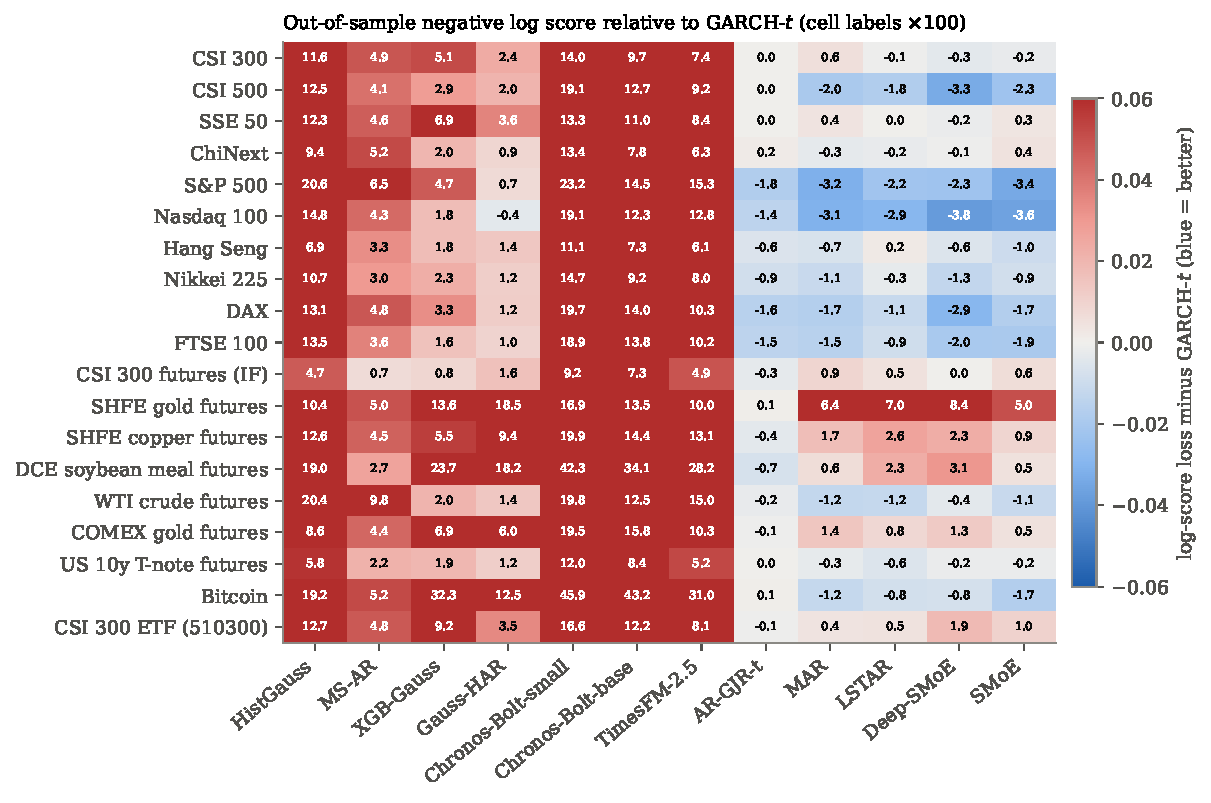
\includegraphics[width=\textwidth]{../results/figures/heatmap_nll.pdf}
\caption{Out-of-sample log-score loss of every model minus that of GARCH-$t$, by series (blue: better
than GARCH-$t$; red: worse; cell labels $\times100$). The two leftmost blocks of columns are dominated
by every mixture model; the SMoE, the MAR, the LSTAR and the deep SMoE are blue on most equity
series.}\label{fig:heatmap}
\end{figure}

We draw two conclusions. First, most of the gain of a mixture over a single Gaussian comes from the
\emph{shape} and \emph{variance dynamics} of the predictive distribution: the constant-weight MAR
already captures much of it, and the observable gate adds a small but frequently significant
increment. Second, the white-box SMoE is statistically indistinguishable from its black-box
counterpart in most markets, a finding we make precise with the yardstick in \cref{sec:yardstick}.

\subsection{Which parts of the SMoE matter?}
\Cref{tab:ablation} removes one component at a time and re-runs the walk-forward on eight series.
The components rank clearly. Removing the variance dynamics (constant expert variances) does the most
damage: the full model is significantly better on log score for six of eight
series and on QLIKE for seven, and never worse. Dropping the short-horizon expert ($K=2$) costs log
score significantly on four series and improves it on one. Removing the semantic exclusion restrictions (letting every expert see every
covariate) never improves log score and worsens it on three series: the restrictions buy
identification and interpretability at no predictive cost. Finally, a gate driven by volatility alone
is statistically indistinguishable from the full three-variable gate, in line with the in-sample Wald
tests; a parsimonious practitioner would use it.

\begin{table}[!htbp]\centering\small
\caption{Out-of-sample ablations of the SMoE on eight series (variant minus full model; positive = variant worse)}\label{tab:ablation}
\begin{adjustbox}{max width=\textwidth}
\begin{tabular}{llrrr}
\toprule
Variant & Loss & Median loss difference & Full SMoE significantly better & Full SMoE significantly worse\\
\midrule
SMoE-K2 & CRPS & -0.0002 & 1 & 0\\
SMoE-K2 & FZ5 & 0.0059 & 2 & 0\\
SMoE-K2 & NLL & 0.0039 & 4 & 1\\
SMoE-K2 & QLIKE & 0.0027 & 3 & 1\\
SMoE-constvar & CRPS & 0.0044 & 4 & 0\\
SMoE-constvar & FZ5 & 0.0210 & 4 & 0\\
SMoE-constvar & NLL & 0.0161 & 6 & 0\\
SMoE-constvar & QLIKE & 0.0369 & 7 & 0\\
SMoE-unrestricted & CRPS & 0.0004 & 1 & 1\\
SMoE-unrestricted & FZ5 & -0.0037 & 1 & 0\\
SMoE-unrestricted & NLL & 0.0031 & 3 & 0\\
SMoE-unrestricted & QLIKE & -0.0024 & 1 & 0\\
SMoE-volgate & CRPS & -0.0000 & 1 & 0\\
SMoE-volgate & FZ5 & -0.0034 & 1 & 2\\
SMoE-volgate & NLL & 0.0025 & 1 & 0\\
SMoE-volgate & QLIKE & -0.0019 & 2 & 1\\
\bottomrule
\end{tabular}
\end{adjustbox}
\par\smallskip\begin{minipage}{\textwidth}\footnotesize
Series: CSI 300, CSI 500, SSE 50, ChiNext, S\&P 500, Hang Seng, COMEX gold, Bitcoin. Counts of series with one-sided DM-HLN $p<0.05$ in favour of the full model and two-sided $p<0.05$ against it.
\end{minipage}
\end{table}

\subsection{Means and directions}
Consistent with \cref{sec:lagging} and with \citet{welch2008comprehensive}, no model forecasts daily
means reliably. The median out-of-sample $R^2$ against a zero forecast is negative for every model,
between $-0.07\%$ (AR-GJR-$t$) and $-2.3\%$ (TimesFM-2.5). The Clark--West test rejects at 5\% for the SMoE on three series (S\&P~500,
Nasdaq~100, DCE soybean meal) and the hit rate averages $50.9\%$. On squared error and Brier score the
simplest models rank best. In daily data, a distributional model earns its keep in risk forecasts;
it does not forecast direction.


\subsection{Calibration}
Calibration is where the SMoE separates from the GARCH family. Its 1\% VaR passes the Kupiec test on
17 of 19 series (GARCH-$t$: 10; historical Gaussian: 1) and its average 1\% violation rate is
$0.97\%$. At 5\% the SMoE is slightly conservative (average violation rate $4.2\%$), which the
conformal layer corrects (\cref{sec:conformal-results}). The PIT standard deviation is $0.97$, close to
the ideal of one. The Chronos-Bolt models have average PIT standard deviations of $1.25$ and $1.32$,
i.e.\ their predictive distributions are far too narrow, which explains their poor log scores
(\cref{fig:pit}). TimesFM~2.5 is better calibrated ($1.17$) but still too narrow: its 1\% VaR is
violated on $3.1\%$ of days on average and fails the Kupiec test on every series, as do both
Chronos models.


\begin{figure}[t]\centering
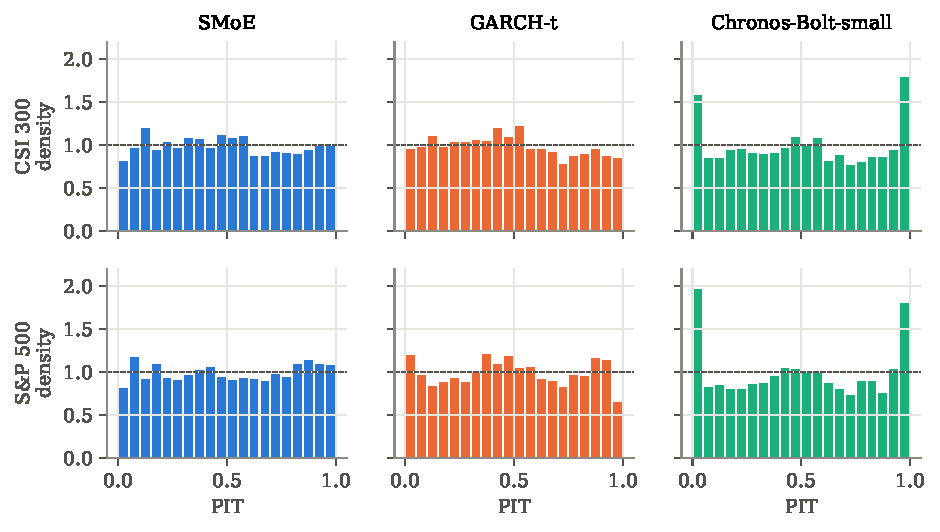
\includegraphics[width=\textwidth]{../results/figures/pit_hist.pdf}
\caption{Probability integral transforms of out-of-sample forecasts. A calibrated forecaster has a
flat histogram (dashed line). The foundation model's U shape shows predictive distributions that are
too narrow.}\label{fig:pit}
\end{figure}

\subsection{Cross-market white-box fingerprints}
\Cref{tab:fingerprints} collects the key SMoE coefficients for every series and
\cref{fig:fingerprints} plots their robust $t$-statistics.

\begin{figure}[t]\centering
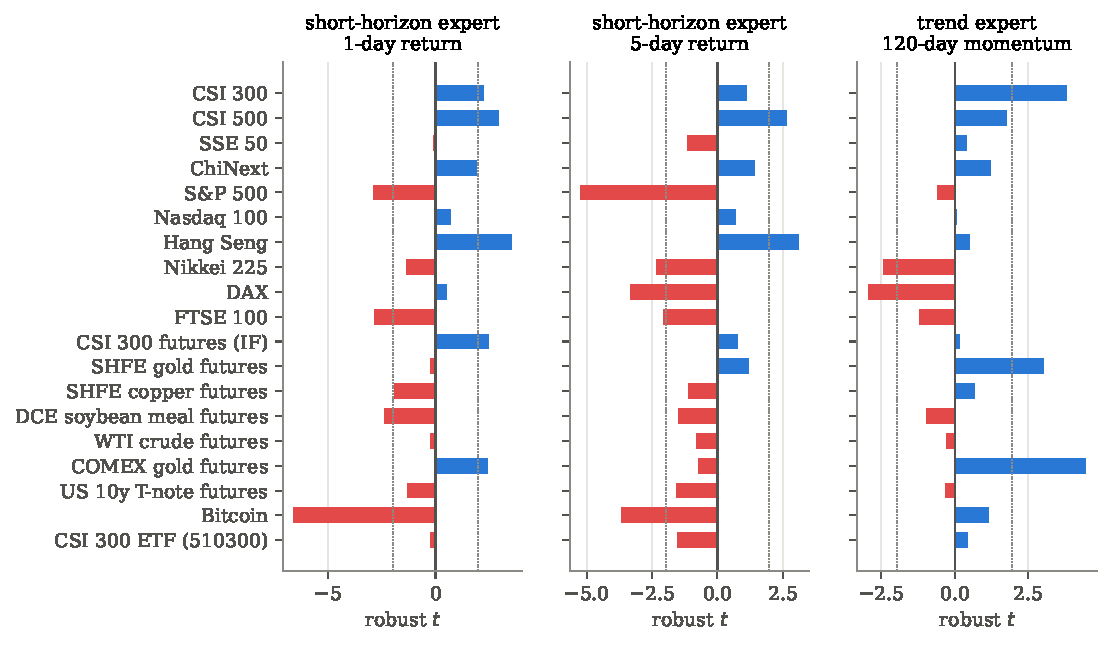
\includegraphics[width=\textwidth]{../results/figures/fingerprints.pdf}
\caption{White-box fingerprints: robust $t$-statistics of the short-horizon expert's loadings on the
scaled 1- and 5-day returns and of the trend expert's loading on 120-day momentum, by series. Dotted
lines mark $\pm1.96$.}\label{fig:fingerprints}
\end{figure} The pattern of the
short-horizon expert is the clearest cross-market regularity in the paper. In the Chinese equity
indices the scaled one-day return enters with a \emph{positive} sign (CSI~300 $z=2.2$, CSI~500
$z=2.9$, ChiNext $z=1.9$), while the five-day scaled return is \emph{negative} and highly significant
in the S\&P~500 ($z=-5.2$), the DAX ($z=-3.3$), the Nikkei ($z=-2.3$) and the FTSE ($z=-2.1$).
Short-horizon continuation in China and short-horizon reversal in developed markets is consistent with
the dominance of retail order flow in the A-share market \citep{liu2019size}; in the SMoE it is not an
unconditional autocorrelation but a property of a specific, high-variance regime, with a
standard error. Slow momentum is equally market-specific: 120-day momentum enters the trend expert
positively and significantly for CSI~300 ($z=3.8$) and both gold contracts ($z=3.0$ and $4.5$), but
negatively for the Nikkei and the DAX ($z=-2.4$ and $-3.0$), where the trend regime is better
described by 20-day momentum.
